\documentclass[11pt,a4paper]{article}

\usepackage[T1]{fontenc}
\usepackage[utf8]{inputenc}
\usepackage{lmodern}
\usepackage{microtype}
\usepackage[margin=2.5cm]{geometry}
\usepackage{amsmath,amssymb}
\usepackage{booktabs}
\usepackage{array}
\usepackage{graphicx}
\usepackage[font=small,labelfont=bf]{caption}
\usepackage[round]{natbib}
\usepackage[hidelinks]{hyperref}
\usepackage[capitalise,noabbrev]{cleveref}
\usepackage{titlesec}
\titlespacing*{\section}{0pt}{2.2ex plus 0.5ex}{1.1ex}
\titlespacing*{\subsection}{0pt}{1.8ex plus 0.5ex}{0.8ex}
\titlespacing*{\paragraph}{0pt}{1.2ex plus 0.3ex}{0.8em}
\setlength{\abovecaptionskip}{4pt}
\setlength{\textfloatsep}{12pt plus 2pt minus 4pt}

\setlength{\bibsep}{1pt}
\renewcommand{\bibfont}{\footnotesize}
\renewcommand{\topfraction}{0.9}
\renewcommand{\bottomfraction}{0.8}
\renewcommand{\textfraction}{0.1}
\renewcommand{\floatpagefraction}{0.8}
\setcounter{topnumber}{3}
\setcounter{totalnumber}{4}
% page ranges in the bibliography: BibTeX sees the hyphen in the argument (so it writes
% "pages"), and the page shows one plain hyphen, not the dash BibTeX would make of it
\newcommand{\hyph}[1]{-}
\graphicspath{{../results/figures/}}
\newcommand{\nOrders}{40,501}
\newcommand{\nDropWeight}{4}
\newcommand{\nDropCoord}{14}
\newcommand{\nPrefixDropCoord}{13}
\newcommand{\nPrefixes}{5,545}
\newcommand{\warehouseSellers}{49}
\newcommand{\foldStart}{2017-08-07}
\newcommand{\foldWeeks}{52}
\newcommand{\osrmPoints}{420}
\newcommand{\osrmRequests}{81}
\newcommand{\osrmBlock}{50}
\newcommand{\osrmDate}{2026-09-24}
\newcommand{\holdingValue}{0.0205}
\newcommand{\vanCapacity}{650}
\newcommand{\nSeeds}{10}
\newcommand{\limitSmall}{10}
\newcommand{\limitMedium}{60}
\newcommand{\limitLarge}{120}
\newcommand{\limitGurobi}{600}
\newcommand{\nWorkers}{4}
\newcommand{\nThreads}{1}
\newcommand{\alphaLevel}{0.05}
\newcommand{\nCpus}{8}
\newcommand{\gurobiVersion}{13.0.3}
\newcommand{\pythonVersion}{3.12.13}
\newcommand{\nRuns}{466}
\newcommand{\nGurobiOptimal}{12}
\newcommand{\nSmall}{12}
\newcommand{\gurobiMaxTime}{111.6}
\newcommand{\gurobiTotalTime}{195.6}
\newcommand{\greedyMaxGap}{4.87}
\newcommand{\greedyMinGap}{0.00}
\newcommand{\greedyMaxVanGap}{20.66}
\newcommand{\greedyMinGapCompare}{5.07}
\newcommand{\greedyMaxGapCompare}{19.18}
\newcommand{\alnsMaxGapCompare}{6.16}
\newcommand{\mhMaxGapCompare}{0.63}
\newcommand{\pGreedyMax}{0.0020}
\newcommand{\pExactMin}{0.0020}
\newcommand{\pEachMin}{0.1934}
\newcommand{\pEachMax}{0.6953}
\newcommand{\lpCallsLarge}{6,032}
\newcommand{\lpRescuesLarge}{6,025}
\newcommand{\lpCallsOther}{0}
\newcommand{\lpMeanMin}{180.5}
\newcommand{\lpMeanMax}{220.8}
\newcommand{\lpRunMin}{25}
\newcommand{\lpRunMax}{628}
\newcommand{\rejectedAlnsLarge}{39.8}
\newcommand{\rejectedMhLarge}{0.23}
\newcommand{\holdingShareBase}{0.27}
\newcommand{\peakMediumMax}{444.1}
\newcommand{\peakLargeMin}{780.5}
\newcommand{\peakLargeMax}{901.1}
\newcommand{\sensTripsBase}{6.0}
\newcommand{\sensTripsHigh}{13.0}
\newcommand{\sensTripsTop}{17.7}
\newcommand{\sensVisitsBase}{261.7}
\newcommand{\sensVisitsMid}{270.7}
\newcommand{\sensVisitsHigh}{353.8}
\newcommand{\sensVisitsTop}{431.1}
\newcommand{\stdAlnsMedium}{780.21}
\newcommand{\stdMhMedium}{18.72}
\newcommand{\stdAlnsLarge}{1,052.65}
\newcommand{\stdMhLarge}{93.95}
\newcommand{\hubKmMin}{253.1}
\newcommand{\hubKmMax}{421.6}
\newcommand{\tripCostMin}{2,467.55}
\newcommand{\tripCostMax}{3,810.10}

\makeatletter
% the body rows of a table; the TeX primitive keeps \bottomrule working after it
\newcommand{\tablebody}[1]{\@@input tables/#1.tex }
\makeatother

\title{Two-echelon inventory routing on real e-commerce orders from S\~ao Paulo state:
a reproducible benchmark and a comparison of exact and heuristic methods}
\author{Mohammad Hajibabaie\\TU Clausthal}
\date{}

\begin{document}
\maketitle

\begin{abstract}
\noindent
This report studies a two-echelon inventory routing problem (2E-IRP) built from public order data
of the Brazilian marketplace Olist: trucks bring goods from a central warehouse to regional hubs,
vans deliver from the hubs to demand points over several days, and no point may run out of stock. We derive 19 instances from \nOrders{} delivered orders in S\~ao Paulo state, with road
distances from OSRM and costs taken from Brazilian freight tables. One independent checker scores four methods: a mixed-integer program solved by Gurobi, a greedy
baseline, an adaptive large neighborhood search (ALNS), and a matheuristic that adds a linear
program for the quantities to the ALNS. Gurobi proves optimality on all \nSmall{}
small instances, and both the ALNS and the matheuristic reach the optimum in every one of
\nSeeds{} runs per instance. On the medium and large instances both heuristics beat the greedy
baseline in every run (Wilcoxon signed-rank test, $p = \pGreedyMax$ on each instance), while the
difference between the ALNS and the matheuristic is not significant on any instance. The linear
program is called only when the just-in-time quantity rule overloads a van, and in our runs this
happened on the large instances only.

\end{abstract}

\section{Introduction}\label{sec:intro}

In an inventory routing problem (IRP) one supplier decides, for every period of a horizon, which
customers to visit, in which order, and how much to deliver, so that no customer runs out of
stock and the sum of routing and holding costs is as small as possible
\citep{archetti2007branch,coelho2014thirty}. The two-echelon version adds a middle layer: large
vehicles bring goods from a central warehouse to intermediate depots, and smaller vehicles serve
the customers from there. The survey of \citet{cuda2015survey} names city logistics as the main motivating example of
two-echelon distribution. In that setting, large trucks stay outside the dense urban area and small
vehicles serve it.

E-commerce last-mile delivery has this structure. Orders arrive every day at many small addresses,
a long-haul leg connects the sellers to the metropolitan areas, and short van routes serve the
local pickup points. When the carrier also controls the stock at the pickup points, it can trade
fewer and fuller deliveries against the cost of the goods waiting in stock. This trade-off is the
one the IRP models.

The 2E-IRP instances of \citet{charaf2024branch} are generated from the single-echelon IRP
benchmark of \citet{archetti2007branch} by placing satellites and suppliers on rings around the
customer area. This project builds a small benchmark from real order data instead. It
contributes a reproducible pipeline from the public Olist dataset \citep{olist2021dataset} to 19
frozen 2E-IRP instances with road distances and sourced costs, and a comparison of an exact mixed-integer program (MIP), a greedy rule, an ALNS and an
ALNS-based matheuristic on them, with every solution verified by one independent checker.

\section{Related work}\label{sec:related}

\paragraph{Inventory routing.}
\citet{archetti2007branch} give a branch-and-cut algorithm for the single-vehicle IRP and compare
the order-up-to policy with the maximum-level (ML) policy, under which any quantity up to the
customer capacity may be delivered. \citet{coelho2014thirty} survey and classify IRP variants. Exact methods for
multi-vehicle IRPs include the branch-and-cut of \citet{coelho2013exact} and the formulations of
\citet{adulyasak2014formulations}, who find that formulations with a vehicle index and symmetry
breaking are better at finding optimal solutions. \citet{solyali2011branch}
propose a strong formulation of the replenishment part under the order-up-to policy.

\paragraph{Two-echelon inventory routing.}
\citet{guimaraes2019two} study a two-echelon multi-depot IRP and solve it with a matheuristic in
which a metaheuristic handles the vehicle routes and a subproblem is solved exactly.
\citet{farias2021model} formulate a 2E-IRP with routing at both levels, solve it by branch-and-cut
with valid inequalities, and add a two-step matheuristic. \citet{rohmer2019two} combine an ALNS with
a reduced formulation for a two-echelon IRP of perishable products. \citet{charaf2024branch} solve
the 2E-IRP by branch-and-price, and \citet{charaf2024matheuristic} combine tabu search with
mathematical programming models. We take the order of operations within one period from
\citet{charaf2024branch}.

\paragraph{Large neighborhood search and matheuristics.}
Large neighborhood search removes a part of a solution and inserts it again
\citep{shaw1998using}. \citet{ropke2006adaptive} add adaptive weights that select among several
removal and insertion heuristics, and \citet{pisinger2007general} apply the same framework to
several vehicle routing problems. \citet{voigt2025review} ranks ALNS operators in a meta-analysis of published
studies; sequence-based removal ranks best among the removal operators and regret insertion among
the insertion operators.
\citet{coelho2012consistency} solve a multi-vehicle IRP by an ALNS in which some subproblems are
solved exactly. \citet{coelho2012transshipment} solve a single-vehicle IRP with transshipment by an
ALNS; once the routes are fixed, a minimum cost network flow sets all quantities and stocks.
\citet{archetti2012hybrid} and \citet{archetti2017matheuristic} combine tabu search with MIP
models, and \citet{solyali2022effective} solve a sequence of MILPs built from the problem
formulation. Our matheuristic follows the route-then-quantity split of
\citet{coelho2012transshipment}.

\section{Problem and MIP formulation}\label{sec:model}

A central warehouse (node 0) supplies $k$ hubs. Each demand point belongs to one fixed hub, its
nearest one. In each day of the horizon the following happens in this order
\citep{charaf2024branch}: trucks bring goods from the warehouse to hubs, vans load at the hubs and
deliver to the demand points, the points consume the demand of the day, and holding cost is charged
on the stock left at the end of the day. Goods that reach a hub in the morning may leave on a van
on the same day. The warehouse has unlimited stock and no holding cost. Stocks follow the ML policy.

The first echelon uses direct trips: a truck drives from the warehouse to one hub and back, at most
once per hub and day. Trucks are hired per trip, so the fleet is not limited. A trip to hub $h$
costs $g_h = f^1 + 2c^1\delta_{0h}$, a fixed charge plus the per-km rate on both legs. Each hub has
$m$ vans. A van drives at most one route per day, and each point is visited at most once per day,
by one van.

\paragraph{Sets and parameters.}
$H$ is the set of hubs, $N_h$ the points of hub $h$, $N = \bigcup_h N_h$, and
$\mathcal{T} = \{0,\dots,T-1\}$ the days. $B = \{1,\dots,m\}$ indexes the vans of each hub.
$V_h = \{h\} \cup N_h$ and $A_h = \{(a,c) \in V_h \times V_h : a \ne c\}$ are the nodes and arcs
of hub $h$. $d_{it}$ is the demand of point $i$ on day $t$, $U_i$ and $C_h$ are the capacities of
point $i$ and hub $h$, and $I^0_i$ and $I^0_h$ are the initial stocks. $Q^1$ and $Q^2$ are the truck
and van capacities, $c^1$ and $f^1$ the truck cost per km and per trip, $c^2$ the van cost per km,
$\delta_{ac}$ the road distance in km, and $\eta^H$ and $\eta^P$ the holding costs per kg and day at
hubs and points.

\paragraph{Variables.}
$z_{ht} \in \{0,1\}$ is 1 if a truck drives to hub $h$ on day $t$, and $y_{ht} \ge 0$ is the
quantity it brings. For van $b$ of hub $h$ on day $t$: $x_{acbt} \in \{0,1\}$ is 1 if the van
drives arc $(a,c) \in A_h$, $v_{ibt} \in \{0,1\}$ is 1 if it visits point $i \in N_h$,
$w_{hbt} \in \{0,1\}$ is 1 if it is used, $q_{ibt} \ge 0$ is the quantity it delivers to point
$i$, and $u_{ibt} \in [1, |N_h|]$ is the position of point $i$ on its route. $I_{ht} \ge 0$ and
$I_{it} \ge 0$ are the end-of-day stocks, with $I_{h,-1} = I^0_h$ and $I_{i,-1} = I^0_i$.

\paragraph{Model.}
In the index sets below, $h \in H$, $i, j \in N_h$, $b \in B$ and $t \in \mathcal{T}$.
\begin{align}
\min\ & \sum_{t \in \mathcal{T}} \sum_{h \in H} g_h z_{ht}
  + c^2 \sum_{h \in H} \sum_{b \in B} \sum_{t \in \mathcal{T}} \sum_{(a,c) \in A_h}
    \delta_{ac} x_{acbt} \notag\\
  & + \sum_{t \in \mathcal{T}} \Big( \eta^H \sum_{h \in H} I_{ht}
    + \eta^P \sum_{i \in N} I_{it} \Big) \label{eq:obj}\\
\text{s.t.}\ & y_{ht} \le \min(C_h, Q^1)\, z_{ht} && \forall h, t \label{eq:trip}\\
& I_{h,t-1} + y_{ht} \le C_h && \forall h, t \label{eq:hubmax}\\
& I_{ht} = I_{h,t-1} + y_{ht} - \sum_{i \in N_h} \sum_{b \in B} q_{ibt}
  && \forall h, t \label{eq:hubbal}\\
& I_{i,t-1} + \sum_{b \in B} q_{ibt} \le U_i && \forall h, i, t \label{eq:pointmax}\\
& I_{it} = I_{i,t-1} + \sum_{b \in B} q_{ibt} - d_{it} && \forall h, i, t \label{eq:pointbal}\\
& \sum_{b \in B} v_{ibt} \le 1 && \forall h, i, t \label{eq:onevan}\\
& \sum_{c \in V_h \setminus \{i\}} x_{icbt} = v_{ibt},\quad
  \sum_{c \in V_h \setminus \{i\}} x_{cibt} = v_{ibt} && \forall h, i, b, t \label{eq:degree}\\
& \sum_{j \in N_h} x_{hjbt} = w_{hbt},\quad \sum_{j \in N_h} x_{jhbt} = w_{hbt}
  && \forall h, b, t \label{eq:depot}\\
& q_{ibt} \le \min(U_i, Q^2)\, v_{ibt} && \forall h, i, b, t \label{eq:visitq}\\
& \sum_{i \in N_h} q_{ibt} \le Q^2 w_{hbt} && \forall h, b, t \label{eq:vancap}\\
& u_{jbt} \ge u_{ibt} + 1 - |N_h| (1 - x_{ijbt}) && \forall h, i \ne j, b, t \label{eq:mtz}\\
& w_{hbt} \le w_{h,b-1,t} && \forall h, t,\ b \ge 2 \label{eq:sym}
\end{align}

The objective \eqref{eq:obj} adds the truck trip, van routing and holding costs.
Constraint \eqref{eq:trip} allows a shipment to a hub only on a trip day.
Constraint \eqref{eq:hubmax} is the ML policy at a hub: the stock before van loading plus the
truck delivery fits in the hub. Constraint \eqref{eq:hubbal} is the hub stock balance; with
$I_{ht} \ge 0$, vans load only what the hub holds. Constraint \eqref{eq:pointmax} is the ML
policy at a point. Constraint \eqref{eq:pointbal} is the point stock balance, and $I_{it} \ge 0$ is
the no-stockout rule. Constraint \eqref{eq:onevan} lets at most one van visit a point on a day.
Constraint \eqref{eq:degree} gives a visited point one arc in and one arc out, both of the same
van. Constraint \eqref{eq:depot} makes a used van leave its hub once and return once. Constraint
\eqref{eq:visitq} allows a delivery only on a visit. Constraint \eqref{eq:vancap} is the van
capacity and, since only $m$ vans exist, also the fleet limit. Constraint \eqref{eq:mtz} is the
subtour elimination of \citet{miller1960integer}: an arc between two points puts the second one
later on the route, so every cycle passes through the hub. Constraint \eqref{eq:sym} breaks the
symmetry of identical vans: van $b$ runs only if van $b-1$ runs.

The model is implemented in \texttt{gurobipy} with \texttt{MIPGap} 0, one thread, and
\texttt{IntegralityFocus} 1. The last setting matters for correctness: Gurobi accepts a binary
variable up to $10^{-5}$ away from an integer, and through \eqref{eq:visitq} a value of $v_{ibt}$
read as 0 could otherwise carry a small positive delivery that the checker rejects. Binaries are
rounded when the solution is read back, and the objective value is compared with the cost the
checker computes (\cref{sec:checker}).

\section{Data and instances}\label{sec:data}

\paragraph{Orders.}
The Olist dataset \citep{olist2021dataset} contains orders of a Brazilian marketplace from 2016 to
2018. We keep orders of customers in S\~ao Paulo state (SP) with status \emph{delivered}:
\nOrders{} orders that have at least one item. The weight of an order is the sum of the product
weights of its items, and its date is the purchase date. We drop \nDropWeight{} orders with a
missing item weight. Each zip code prefix (five digits) is placed at the median latitude and
longitude of its geolocation rows inside an SP bounding box. \nPrefixDropCoord{} prefixes without a coordinate (\nDropCoord{}
orders) are dropped, which leaves \nPrefixes{} prefixes.

\paragraph{Demand folding.}
A single real week is too thin for an IRP: most prefixes order nothing on most days. We therefore
fold one year of orders onto one week. The demand of prefix $i$ on weekday $t$ is the total weight of
its orders placed on that weekday during the \foldWeeks{} weeks that start on Monday \foldStart{}.
Each demand point is thus a pickup point that receives one year of its zip area's orders
within one week. The day-to-day variation is real, and the only scale parameter is the
number of folded weeks.

\paragraph{Warehouse and hubs.}
The warehouse is the seller zip prefix with the most sellers: prefix 14940 in Ibitinga, with
\warehouseSellers{} sellers. The hubs are the SP cities with the largest delivered weight, each
placed at its prefix with the most orders. In this order they are S\~ao Paulo, Campinas, Guarulhos, Santos and S\~ao Bernardo do
Campo, and an instance with $k$ hubs uses the first $k$. On instance
\texttt{large\_k5\_n200\_T7\_s1} the road distance from the warehouse to a hub lies between
\hubKmMin{} and \hubKmMax{}~km, so one truck trip costs between \tripCostMin{} and
\tripCostMax{} BRL. The hub prefix itself is not a demand point, so its own demand is not served.

\paragraph{Demand points.}
For $k$ hubs, the point pool holds every prefix within a straight-line radius of its nearest hub,
excluding the hub prefixes, ranked by the number of orders; the pool keeps the busiest prefixes up
to a fixed size (\cref{tab:params}). An instance draws its $n$ points from the pool with a fixed
seed. Capacities and initial stocks follow four rules. C1: the capacity $U_i$ of a point is the
larger of its busiest folded day and a fixed number of average days. C2: its initial stock is a
fixed number of average days. C3: a hub holds a fixed multiple of the capacities of its points. C4:
the initial stock of a hub is a fixed number of average days of its region. Four build checks make every method able to find a feasible solution: a hub fits in one truck
(A1), the points of a hub fit into $m$ vans under the greedy packing (A2), a point capacity fits
in one van (A3), and every hub has a point (A4).

\paragraph{Road distances.}
Distances come from the table service of the OSRM demo server \citep{luxen2011real}, which returns
the distances of the fastest routes on OpenStreetMap data. One directed matrix over the warehouse,
the five hubs and the union of all point pools (\osrmPoints{} locations) was fetched on
\osrmDate{} in \osrmRequests{} requests of $\osrmBlock \times \osrmBlock$ locations; no location
lacked a route. The distance between two nodes is the mean of both directions. These road distances break the triangle inequality, so the MIP could shorten a route by passing a
point without delivering, which the heuristics never do. Each instance therefore replaces every
distance by the shortest path through its other nodes (the Floyd-Warshall algorithm).

\paragraph{Parameters.}
\Cref{tab:params} lists every parameter with its value and source. The truck is a two-axle truck;
its cost per km and per trip are the minimum freight prices of the Brazilian land transport agency
ANTT for general cargo \citep{antt2026resolucao6084}, charged on both legs of the trip. The van is a
Fiat Fiorino with a payload of \vanCapacity{}~kg; we chose this small urban van because with a
larger van the van capacity never bound on any instance. No official van cost table was found, so
the van reuses the truck rate per km; this is an assumption. The holding cost is the capital cost
of the goods only: the total item price divided by the total item weight of the kept orders in the
fold window, times the Selic policy rate of the Brazilian central bank \citep{bcb2026selic}, divided by 365. It is the same at hubs and points
because the goods are the same, and it is small (\holdingValue{} BRL per kg and day, rounded). The
order data are from 2017 and 2018 while costs and rates are from 2026; no inflation adjustment is
made.

\begin{table}[!tbp]
\centering\footnotesize
\caption{Parameters with value and source. Values are read from \texttt{config/params.toml}; the
holding cost is computed from the goods value and the Selic rate and rounded here to four decimals. ANTT: \citet{antt2026resolucao6084}; BCB: \citet{bcb2026selic}.
The rules C1 to C4 and A2 are described in \cref{sec:data}.}
\label{tab:params}
\begin{tabular}{llrp{6.2cm}}
\toprule
Symbol & Meaning & Value & Source \\
\midrule
\tablebody{parameters}
\bottomrule
\end{tabular}
\end{table}

\paragraph{Instance sets.}
Three sets are built (\cref{tab:instances}). The small set has 1 or 2 hubs, 6 to 10 points and
$T = 3$ days, sized so that Gurobi proves optimality. The large set has all 5 hubs, 200 points and
$T = 7$, in line with the 200-customer scale of IRP benchmarks \citep{archetti2017matheuristic}.
The medium set lies in between. \Cref{fig:map} shows the network of one large instance. The last
column of \cref{tab:instances} is the busiest hub-day: the largest demand of one hub region on one
day. It is at most \peakMediumMax{}~kg on the medium set and between \peakLargeMin{} and
\peakLargeMax{}~kg on the large set, against a van capacity of \vanCapacity{}~kg. On the small
and medium sets one day of demand of a hub region thus fits in one van. A route can still exceed the
van capacity there if its visits bring several days of demand.

\begin{table}[!tbp]
\centering\footnotesize
\caption{The 19 instances. $k$ hubs, $n$ points, $T$ days; points per hub (smallest to largest);
total demand over the horizon (kg); busiest hub-day, the largest one-day demand of one hub region
(kg).}
\label{tab:instances}
\begin{tabular}{lrrrrrr}
\toprule
Instance & $k$ & $n$ & $T$ & Points per hub & Total demand & Busiest hub-day \\
\midrule
\tablebody{instances}
\bottomrule
\end{tabular}
\end{table}

\begin{figure}[!tbp]
\centering
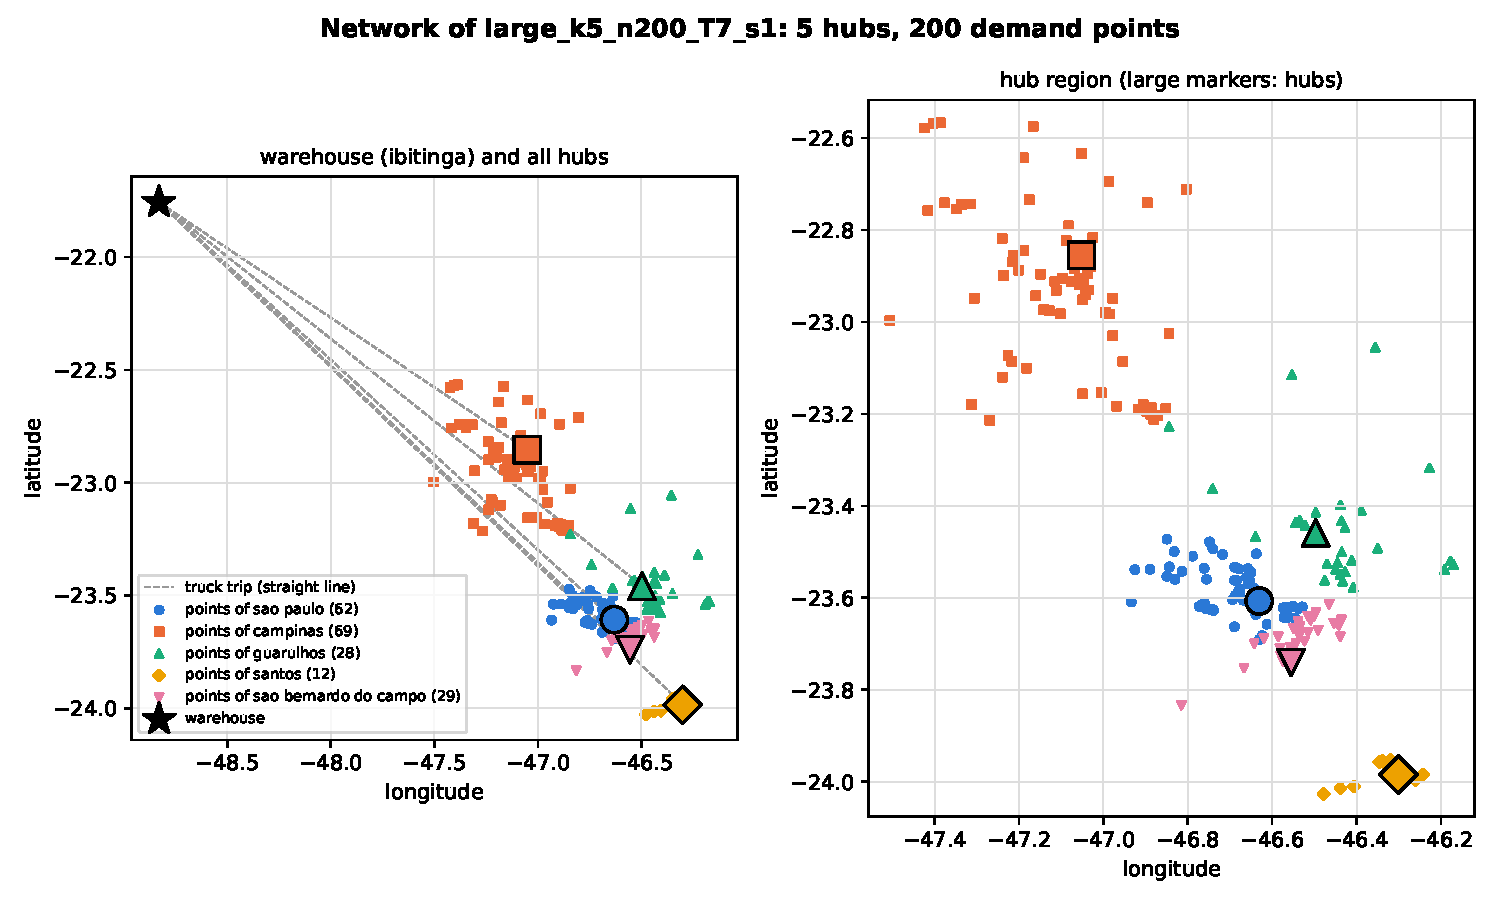
\includegraphics[width=0.66\textwidth]{network_map}
\caption{Network of instance \texttt{large\_k5\_n200\_T7\_s1}. Left: the warehouse in Ibitinga
and the straight lines of the truck trips to the five hubs. Right: the hub region enlarged, with
each point drawn in the color and marker of its hub. Lines are straight, not road geometry.}
\label{fig:map}
\end{figure}

\section{Methods}\label{sec:methods}

In the ALNS and the matheuristic a \emph{plan} fixes the truck trips and the van routes, and the
quantities follow from the plan by a rule. The greedy rule works the other way round: it sets the
quantities first and builds the routes and truck trips from them.

\subsection{Greedy baseline}\label{sec:greedy}
The greedy rule processes the days in order. G1: a point receives a delivery only if its stock at
the start of the day is below the demand of the day; it is then filled up, but never above what it
still needs until the end of the horizon, $q_{it} = \min(U_i, \sum_{t' \ge t} d_{it'}) - I_{i,t-1}$.
G2: for each hub and day, the points with a delivery are routed by nearest neighbor; a van goes to
the nearest unrouted point whose delivery fits in its remaining capacity, and when no point fits,
the next van starts. G3: a hub is refilled by the same rule as G1, applied to its outflow, the sum of
its points' deliveries. G4: a truck drives to every hub with a positive shipment. The capacity
rules C1 and C3 make G1 and G3 always feasible, and check A2 bounds the number of vans.

\subsection{Adaptive large neighborhood search}\label{sec:alns}

\paragraph{Representation and quantities.}
The search state is a plan: a Boolean truck trip for every hub and day, and a list of routes for
every hub and day. Quantities are not part of the state. They are computed after every change by
the just-in-time rule J1. For one point with visit days $v_1 < \dots < v_r$ and running stock $s$,
a visit on day $v_j$ delivers
\begin{equation}
q = \max\Big(0,\ \min\big(\textstyle\sum_{t=v_j}^{v_{j+1}-1} d_{it} - s,\ U_i - s\big)\Big),
\label{eq:jit}
\end{equation}
the demand up to the day before the next visit (or to the last day), limited by the capacity. The
same rule sets the hub shipments, with the truck trip days as visit days and the hub outflow as
demand. J1 reports the first stockout day of a point or hub. The quantity step returns no answer
when any point or hub runs out or any route carries more than $Q^2$. J1 delivers as late as
possible. When J1 is feasible and $\eta^P \ge \eta^H$, it therefore gives the lowest holding cost
of all quantities that fit the plan: each partial sum of shipments is as small as the plan allows. The search starts from an empty
plan, to which the greedy repair operator below adds every needed visit and truck trip.

\paragraph{Destroy operators.}
Each iteration draws the removal count $\rho$ uniformly from $1,\dots,\rho_{\max}$, where
$\rho_{\max}$ is a share of the current number of visits, clipped to fixed bounds
(\cref{tab:params}). Six destroy operators change the plan. \emph{Random removal} removes $\rho$
visits chosen uniformly. \emph{Worst removal} ranks all visits by the km saved when they are
removed, and removes $\rho$ visits drawn from the top $2\rho$. \emph{Related removal} picks one
visit and removes the $\rho$ visits of the same hub, on any day, whose points are closest to its
point \citep{shaw1998using}; the point's own visits on other days come first. \emph{Sequence
removal} removes up to $\rho$ consecutive stops from one random route \citep{voigt2025review}.
\emph{Hub-day removal} removes all visits of one random hub on one day. \emph{Truck trip removal}
removes one random truck trip; if the previous trip of that hub cannot cover the extra days, the
repair adds a later trip.

\paragraph{Repair.}
Every repair operator first applies rule R-points and ends with rule R-hubs. R-points computes J1
for all points; each point with a stockout needs one new visit on a day between its last visit
before the stockout and the stockout day. An option is a day in this window together with an
existing route of the hub (at its cheapest insertion position) or a new route if fewer than $m$
routes run that day. Its cost is $c^2$ times the added km, and it is allowed only if the route
load after insertion, with the J1 quantity of the new visit, stays within $Q^2$. The \emph{greedy
repair} inserts the cheapest option over all needy points and repeats. The \emph{regret repair}
inserts first the point with the largest difference between its best and second-best option
\citep{ropke2006adaptive}. The \emph{extra-visits repair} runs the greedy repair and then adds one
visit, on a random day without a visit, for up to $\rho$ of the points the destroy operator
touched. The \emph{extra-trip repair} runs the greedy repair and then adds one truck trip on a
random day for one touched hub; it is the only way a truck trip moves earlier. R-hubs then adds a
truck trip on the first stockout day of every hub until no hub runs out. If a needy point has no
allowed option, the repair fails and the candidate is rejected.

\paragraph{One iteration.}
A destroy and a repair operator are drawn by roulette wheel with probability proportional to their
weights \citep{ropke2006adaptive}. After destroy and repair, the quantity step computes $(q, y)$;
if it gives no answer, the candidate is rejected. Visits and trips with zero quantity are then
removed, and every changed route is improved by 2-opt with first improvement
\citep{croes1958method}. A candidate with cost $f'$ replaces the current solution with cost $f$ if
$f' < f$, or else with probability $\exp(-(f' - f)/\tau)$. The start temperature $\tau_0$ is set so
that a solution a share $w$ worse than the initial solution is accepted with probability one half,
$\tau_0 = w f_0 / \ln 2$ \citep{ropke2006adaptive}. The temperature falls geometrically with the
share $p$ of the time budget used, $\tau = \tau_0 \epsilon^{p}$, where $\epsilon$ is the final
temperature ratio. Tying the cooling to the time used lets one schedule serve fast small
instances and slow large ones.

\paragraph{Adaptive weights.}
Both operators of an iteration receive the same score: one value for a new best solution, a
smaller one for a solution better than the current one, and a still smaller one for a worse
solution that is accepted. After every segment of iterations, the weight of operator $j$ becomes
$w_j (1 - r) + r \pi_j / \theta_j$ \citep{ropke2006adaptive}, where $\pi_j$ is its score and
$\theta_j$ its number of uses in the segment; an unused operator keeps its weight. Segment length,
reaction factor $r$ and scores are those of \citet{coelho2012transshipment} (\cref{tab:params}).

\subsection{Matheuristic}\label{sec:mh}
The matheuristic is the same ALNS with the same operators, parameters and seeds; only
the quantity step differs (rule M1). It first applies J1. Only when J1 gives no answer, Gurobi
solves a linear program (LP) over the quantities of the fixed plan:
\begin{equation}
\min \sum_{t \in \mathcal{T}} \Big( \eta^H \sum_{h \in H} I_{ht} + \eta^P \sum_{i \in N} I_{it} \Big)
\label{eq:lp}
\end{equation}
subject to \eqref{eq:hubmax} to \eqref{eq:pointbal} with one quantity $q_{it}$ per point and day
in place of $\sum_b q_{ibt}$, the bounds $0 \le q_{it} \le \min(U_i, Q^2)$ if $i$ is visited on day
$t$ and $q_{it} = 0$ otherwise, $0 \le y_{ht} \le \min(C_h, Q^1)$ if hub $h$ has a trip on day $t$
and $y_{ht} = 0$ otherwise, and $\sum_{i \in r} q_{it} \le Q^2$ for every route $r$ of day $t$.
Routing cost is fixed by the plan, so the LP minimizes holding cost only. The LP is built once per
run; each call changes the bounds and replaces the route rows. If the LP is infeasible, the
candidate is rejected. Since J1 already has the lowest holding cost whenever it is feasible and
$\eta^P \ge \eta^H$, which holds in every run here (\cref{sec:alns}), the LP can only help when J1 overloads a van: it can move part of a delivery to
an earlier visit of the same point. The run counts the LP calls and the calls that return
quantities (LP rescues).

\subsection{Solution checker}\label{sec:checker}
One checker, separate from all methods, verifies every final solution against the rules of \cref{sec:model} (shipments only on trips, capacities, ML rules, stock balances, one visit per
point and day, at most $m$ routes, deliveries only on visits, no stockout) with a tolerance of
$10^{-4}$ kg, and recomputes the cost. Each run passes
the checker before its solution is saved, and the analysis script checks all \nRuns{} saved
solutions again before it writes any table.

\section{Experimental setup}\label{sec:setup}

All runs used one computer with \nCpus{} logical CPUs, \nWorkers{} runs in parallel, Python
\pythonVersion{} and Gurobi \gurobiVersion{} with \nThreads{} thread per Gurobi call. Gurobi solves
the MIP on the small set with a limit of \limitGurobi{}~s. The greedy rule is deterministic and runs
once per instance. The ALNS and the matheuristic run with each of \nSeeds{} seeds per instance, with
time limits of \limitSmall{}~s (small), \limitMedium{}~s (medium) and \limitLarge{}~s (large). The
sensitivity study runs the greedy rule and the ALNS on \texttt{medium\_k3\_n80\_T7\_s1} with the
holding costs $\eta^H$ and $\eta^P$ multiplied by 1, 10, 100, 1000 and 10000, with the medium time
limit. 

Runs stop on wall-clock time and the temperature depends on the time used, so a run is not
bit-reproducible on another machine: two runs with the same seed diverge once their iteration
speeds differ. For the small set the gap of a run is $100(f - f^*)/f^*$, with $f^*$ the proven
optimum, and the van gap compares the van costs in the same way. For the medium and large sets the
reference is the best cost of any run of any method on that instance.

The heuristics are compared on the medium and large sets by the two-sided Wilcoxon signed-rank test
\citep{wilcoxon1945individual} at level \alphaLevel{}, without correction for multiple tests. The
ALNS and the matheuristic are paired by seed. Since the greedy result is a single number, each
heuristic is compared with it by a one-sample test on the \nSeeds{} differences to the greedy
cost. Costs are rounded to $10^{-6}$ BRL before the test. With \nSeeds{} nonzero differences of
the same sign the exact two-sided p-value is $2 \cdot 2^{-\nSeeds} = \pExactMin$, the smallest
value the test can give with \nSeeds{} pairs.

\section{Results}\label{sec:results}

\subsection{Small instances}
Gurobi proves optimality on \nGurobiOptimal{} of the \nSmall{} small instances
(\cref{tab:small}). The longest proof
takes \gurobiMaxTime{}~s and all \nSmall{} take \gurobiTotalTime{}~s together. The ALNS and the
matheuristic reach the proven optimum in every run on every small instance. The greedy gap lies
between \greedyMinGap{}\,\% and \greedyMaxGap{}\,\%. The van gap of the greedy rule is larger, up
to \greedyMaxVanGap{}\,\%, because the truck trips are a large, fixed share of every small optimum
and the greedy rule uses the same number of trips as the optimum on these instances.

\begin{table}[!tbp]
\centering\footnotesize\setlength{\tabcolsep}{4pt}
\caption{Small instances. Optimum and solution time of Gurobi; gap to the optimum (\%) of the
greedy rule, and its van gap (\%); best and mean gap (\%) of the ALNS and the matheuristic (MH)
over \nSeeds{} seeds. Numbers are rounded for display from \texttt{results/tables/*.csv}.}
\label{tab:small}
\begin{tabular}{lrrrrcc}
\toprule
& Optimum & Gurobi & Greedy & Greedy & ALNS & MH \\
Instance & (BRL) & (s) & gap & van gap & best/mean & best/mean \\
\midrule
\tablebody{small}
\bottomrule
\end{tabular}
\end{table}

\subsection{Medium and large instances}
\Cref{tab:compare} summarizes the costs on the medium and large sets and \cref{fig:gaps} shows the
gap of every run. The mean gap of the greedy rule to the best known cost lies between
\greedyMinGapCompare{}\,\% and \greedyMaxGapCompare{}\,\%. Both heuristics beat the greedy cost in
every run on every instance, and each of these comparisons gives $p = \pGreedyMax$
(\cref{tab:wilcoxon}). The largest gap of any matheuristic run is \mhMaxGapCompare{}\,\%, and that
of any ALNS run is \alnsMaxGapCompare{}\,\%. The ALNS has a few poor runs: on
\texttt{medium\_k3\_n80\_T7\_s2} and \texttt{large\_k5\_n200\_T7\_s2} its standard deviation is
\stdAlnsMedium{} and \stdAlnsLarge{} BRL, against \stdMhMedium{} and \stdMhLarge{} BRL for the
matheuristic. On the medium set the matheuristic never called the LP, so this difference comes from diverging
search paths, not from the LP.

The difference between the ALNS and the matheuristic is not significant on any of the seven
instances; the p-values lie between \pEachMin{} and \pEachMax{}. On the three large instances the
matheuristic has the lower mean cost, but the sign of the median paired difference changes between
instances.

\begin{table}[!tbp]
\centering\footnotesize\setlength{\tabcolsep}{4pt}
\caption{Medium and large instances: best, mean and standard deviation of the total cost (BRL) over
\nSeeds{} seeds; mean and largest gap to the best known cost (\%); mean number of iterations; and
mean number of LP rescues per run of the matheuristic (MH). The greedy rule runs once. Numbers are
rounded for display.}
\label{tab:compare}
\begin{tabular}{llrrrrrrr}
\toprule
& & & & & Mean & Max & & LP \\
Instance & Method & Best & Mean & Std & gap & gap & Iterations & rescues \\
\midrule
\tablebody{compare}
\bottomrule
\end{tabular}
\end{table}

\subsection{When the LP matters}
The matheuristic made \lpCallsOther{} LP calls on the small and medium sets. On the large set it
made \lpCallsLarge{} LP calls in total, of which \lpRescuesLarge{} returned feasible quantities.
The mean number of LP rescues per run lies between \lpMeanMin{} and \lpMeanMax{} per instance, and
between \lpRunMin{} and \lpRunMax{} over single runs. J1 overloads a route when a destroy step
removes a later visit of a point, so that an earlier visit must carry more. Once the matheuristic
accepts a rescued plan, that plan keeps a route that J1 overloads, and every candidate made from it
calls the LP again until that route changes. The ALNS rejects every candidate that J1 overloads. Counting rejections for any reason, it rejected
\rejectedAlnsLarge{} candidates per large run on average, against \rejectedMhLarge{} for the
matheuristic. The rescues gave
no significant cost difference within the time limit, and the matheuristic ran fewer iterations than the ALNS on two of the three large instances
(\cref{tab:compare}).

\begin{table}[!tbp]
\centering\small
\caption{Two-sided Wilcoxon signed-rank tests on the medium and large instances: median cost
difference (BRL) and p-value for ALNS minus greedy, matheuristic (MH) minus greedy, and ALNS minus
MH. A negative median means that the first method is cheaper.}
\label{tab:wilcoxon}
\begin{tabular}{lrrrrrr}
\toprule
& \multicolumn{2}{c}{ALNS $-$ Greedy} & \multicolumn{2}{c}{MH $-$ Greedy}
& \multicolumn{2}{c}{ALNS $-$ MH} \\
\cmidrule(lr){2-3}\cmidrule(lr){4-5}\cmidrule(lr){6-7}
Instance & Median & $p$ & Median & $p$ & Median & $p$ \\
\midrule
\tablebody{wilcoxon}
\bottomrule
\end{tabular}
\end{table}

\begin{figure}[!tbp]
\centering
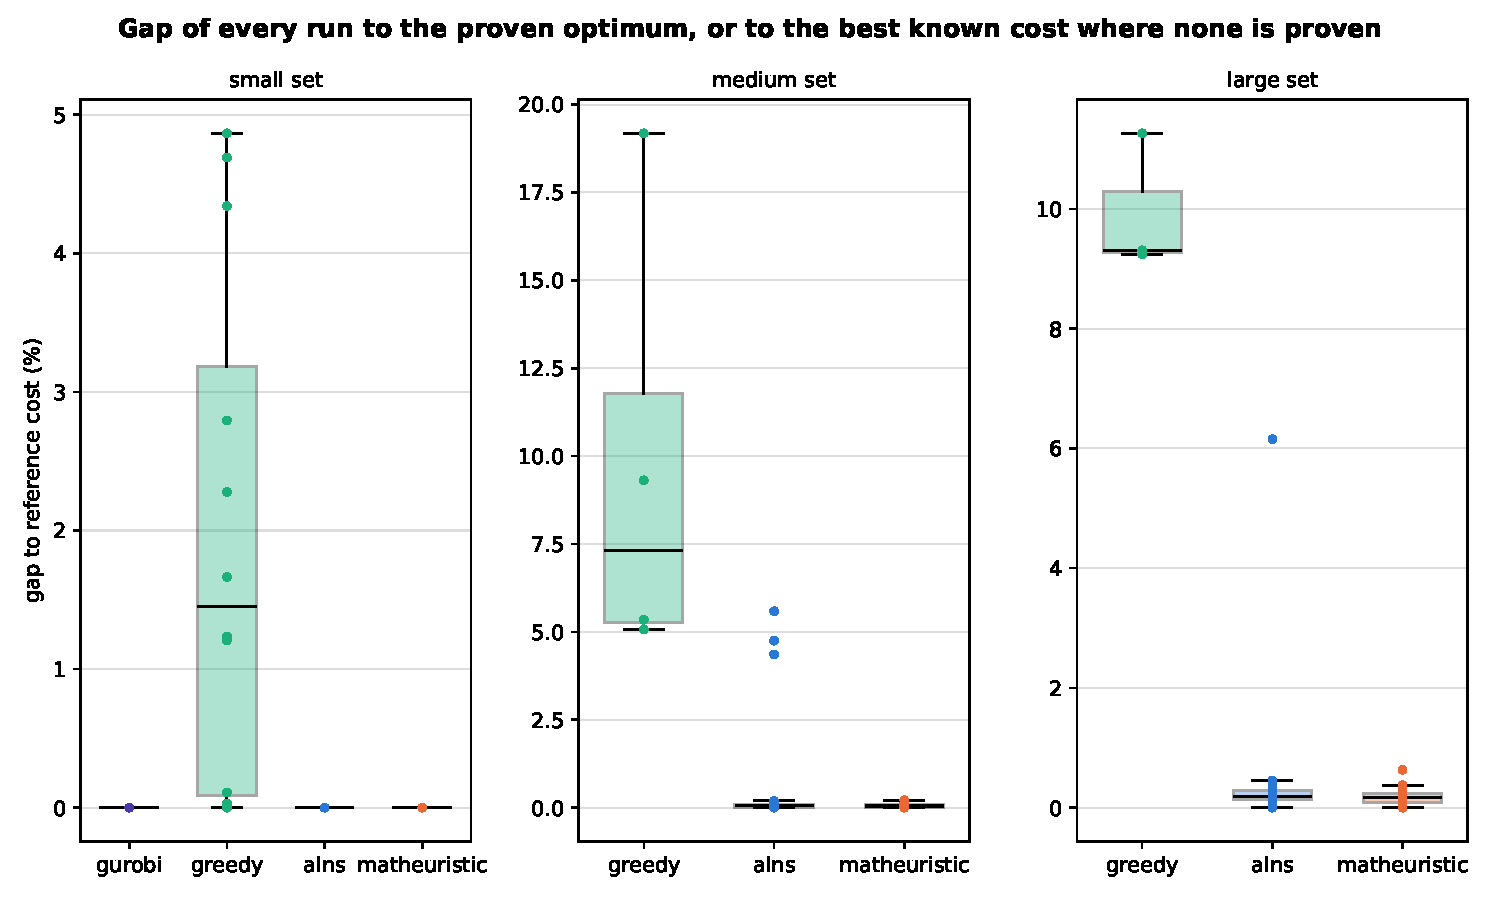
\includegraphics[width=0.66\textwidth]{gap_boxplots}
\caption{Gap of every run to the proven optimum (small set) or to the best known cost of the
instance (medium and large sets). Each dot is one run; boxes show the quartiles.}
\label{fig:gaps}
\end{figure}

\subsection{Holding cost sensitivity}
At the real capital cost, holding is \holdingShareBase{}\,\% of the mean ALNS cost on the
sensitivity instance, and the cost consists almost only of truck trips and van routes
(\cref{tab:sensitivity}, \cref{fig:sensitivity}). Up to a multiplier of 100 the mean number of ALNS truck trips stays at \sensTripsBase{}, and the
mean number of visits rises only from \sensVisitsBase{} to \sensVisitsMid{}. At multipliers 1000 and 10000 the ALNS switches to more frequent and
smaller deliveries: the mean number of truck trips rises to \sensTripsHigh{} and \sensTripsTop{},
and the number of visits from \sensVisitsBase{} to \sensVisitsHigh{} and \sensVisitsTop{}. The greedy rule does not react to the
holding cost at all, so its plan stays the same and its holding cost grows in proportion to the
multiplier. The ALNS is cheaper than the greedy rule at every multiplier, with $p = \pGreedyMax$ in each case.

\begin{table}[!tbp]
\centering\small
\caption{Holding cost sensitivity on \texttt{medium\_k3\_n80\_T7\_s1}: mean total cost and its
parts (BRL), mean number of truck trips and of visits, per holding multiplier. ALNS means are over
\nSeeds{} seeds; the greedy rule runs once. Numbers are rounded for display.}
\label{tab:sensitivity}
\begin{tabular}{rlrrrrrr}
\toprule
Multiplier & Method & Total & Truck & Van & Holding & Trips & Visits \\
\midrule
\tablebody{sensitivity}
\bottomrule
\end{tabular}
\end{table}

\begin{figure}[!tbp]
\centering
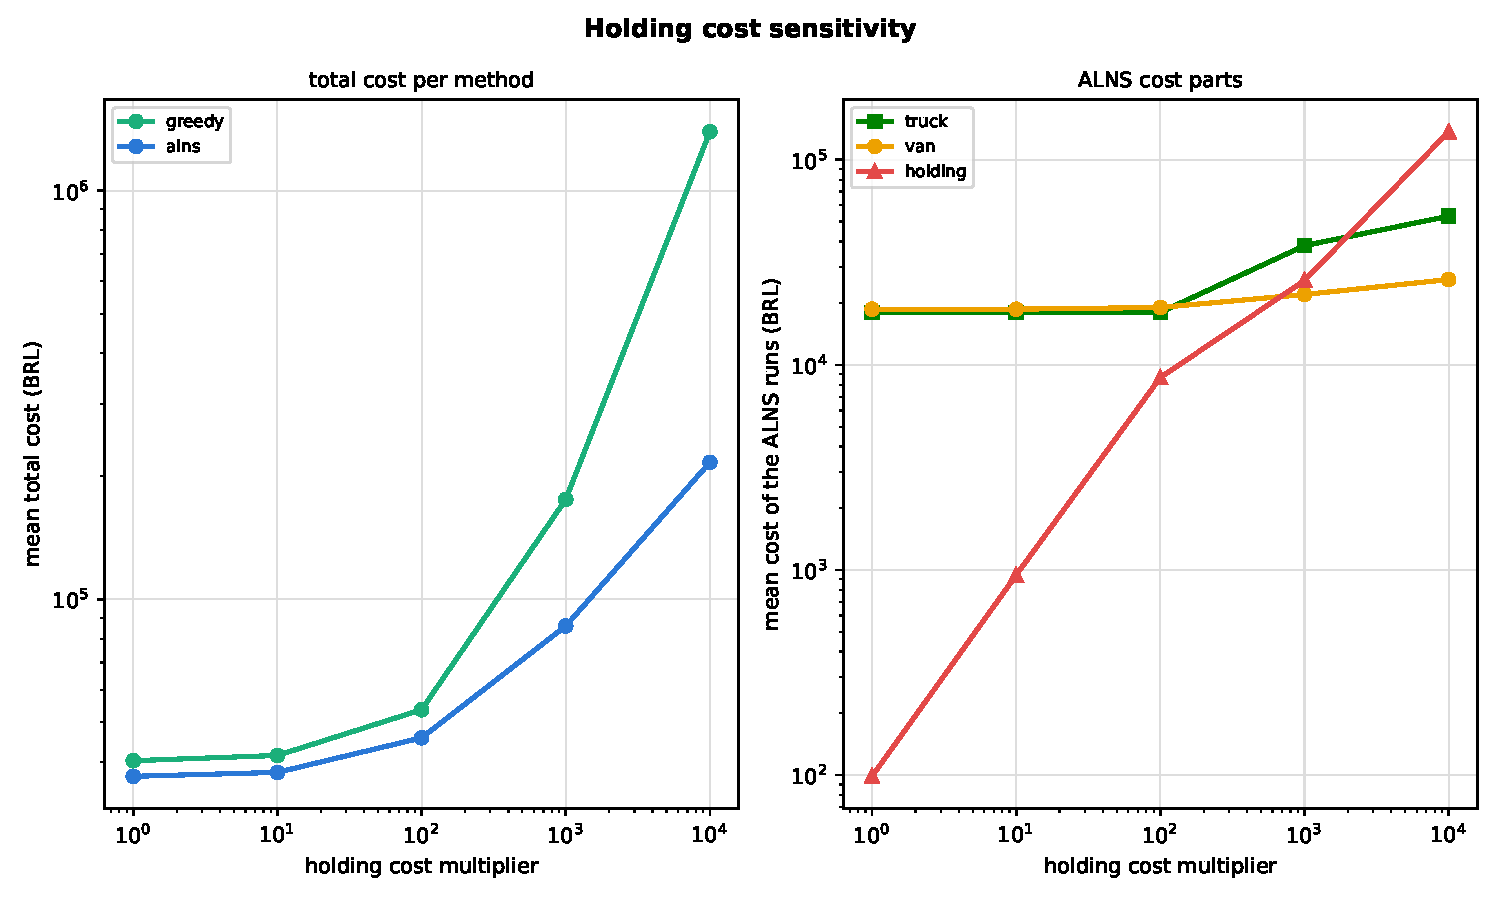
\includegraphics[width=0.66\textwidth]{sensitivity}
\caption{Holding cost sensitivity on \texttt{medium\_k3\_n80\_T7\_s1}. Left: mean total cost of
the greedy rule and the ALNS. Right: mean truck, van and holding cost of the ALNS runs. Both axes
are logarithmic.}
\label{fig:sensitivity}
\end{figure}

\section{Conclusion}\label{sec:conclusion}

On 19 instances built from real Olist orders and road distances, the MIP proves optimality on the
small instances, and the ALNS and the matheuristic find every proven optimum in every run. On the medium and large instances both beat the greedy rule in every run. The LP of the
matheuristic acts only when J1 overloads a van, which in these runs happened only on the large
instances.

The holding cost covers only the capital tied up in stock, so it
is small, and routing decides almost everything at the real value. The first echelon uses direct
trips, although the Guarulhos and S\~ao Bernardo do Campo hubs lie close to the S\~ao Paulo hub, so
one truck tour could serve several hubs. The demand is a year of orders folded onto one week and
is known in advance. The distances come from the public OSRM demo server on one date and are
fastest-route distances. The van cost per km reuses the truck rate. The matheuristic showed no
significant gain, and the operators were not tested one by one, although \citet{voigt2025review}
advises against relying on adaptive selection alone.

Future work follows from these limits: truck tours over several hubs in the first echelon, a
holding cost that includes storage and handling, demand that is uncertain when the plan is made, a
switch-off study (ablation) of each operator, and calling the LP on more plans, for example on
every new best plan when the holding cost is high.

\bibliographystyle{plainnat}
\bibliography{references}

\end{document}
